%  !TeX  root  =  user_guide.tex 

\section{Plugin Testo Delimitato}\label{label_dltext}    

% when the revision of a section has been finalized, 
% comment out the following line:
% \updatedisclaimer

Il plugin permette di caricare un file di testo delimitato come layer in QGIS.

\minisec{Requisiti}

Per visualizzare un file di testo delimitato come layer, il testo deve contenere:

\begin{enumerate}
\item Una riga di intestazione per i nomi dei campi. Questa deve essere la prima riga del file di testo.
\item La riga di intestazione deve contenere un campo X ed uno Y. Questi campi possono avere qualsiasi nome.
\item Le coordinate x e y devono essere specificate come numeri. Il sistema di coordinate non è importante.
\end{enumerate}

Come esempio di un file di testo valido importiamo il file di punti quotati \filename{elevp.csv} presente 
nel dataset campione di QGIS (Sezione~\ref{label_sampledata}):

\begin{verbatim} 
X;Y;ELEV
-300120;7689960;13
-654360;7562040;52
1640;7512840;3
[...]
\end{verbatim}

Alcune note circa il file di testo:

\begin{enumerate}
\item Il file di testo usato come esempio usa \mbox{$;$} (punto e virgola) come delimitatore. Qualsiasi carattere può 
essere usato per delimitare i campi.
\item La prima riga è la riga intestazione. Essa contiene i campi X, Y e ELEV.
\item Nessun tipo di virgoletta (") dev'essere usata per delimitare i campi di testo.
\item Le coordinate x sono contenuto nel campo {\em X}.
\item Le coordinate y sono contenuto nel campo {\em Y}.
\end{enumerate}

\minisec{Utilizzo del plugin}
Attivare il plugin come descritto nella Sezione \ref{sec:managing_plugins}.

Cliccare sulla nuova icona della barra dei plugin \toolbtntwo{delimited_text}{Aggiungi layer di testo delimitato} 
per aprire la finestra di dialogo 'Crea un layer da un file di testo delimitato', mostrata in Figura
\ref{fig:delim_text_plugin_dialog}.

\begin{figure}[ht]
   \centering
   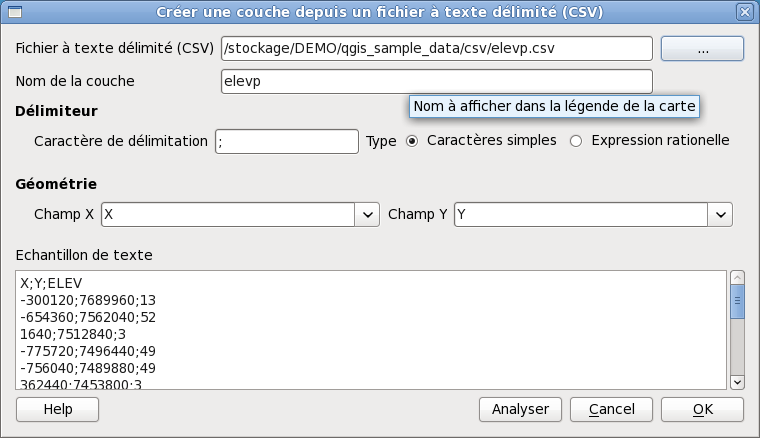
\includegraphics[clip=true, width=10cm]{delimited_text_dialog}   
   \caption{Finestra di dialogo Crea un layer da un file di testo delimitato \nixcaption}\label{fig:delim_text_plugin_dialog}
\end{figure}

Selezionare il file \filename{qgis\_sample\_data/csv/elevp.csv} da importare cliccando su \button{Sfoglia}. 
Una volta caricato il file, il plugin cerca di processarlo usando l'ultimo delimitatore utilizzato, 
in questo caso un punto e virgola (\mbox{$;$}). È fondamentale selezionare il giusto delimitatore. 
Per cambiare delimitatore usare \mbox{$\backslash$}t (questa è un'espressione per il carattere tab).

Selezionare i campi X e Y dai menu a tendina ed il campo WKT per le informazioni sul sistema di riferimento 
(se disponibile). Assegnare un nome al layer (es. \filename{elevp}) ed aggiungere il layer alla vista mappa 
cliccando su \button{OK} (Figura \ref{fig:delim_text_plugin_dialog}).

\FloatBarrier
